\chapter{Background}

\section{Service-oriented Architecture}In this section, we visit the history and definitions used in the Service-oriented Architecture, as well as the emergence of the Microservices Architecture, the state-of-the-art software design in the modern real-world system. At the end of this section, the reader should understand the problem that Jolie programming language is trying to solve.

\textbf{SOA} is a software architecture design that focuses on the composition of services via communication over a network protocol. The majority of SOA implementation realized over Web Services technology, where services are composed together through standard web protocols such as SOAP\cite{Mendelsohn:07:SVP} or HTTP\cite{http-rfc}. In SOA, A service consist of four properties which are \cite{SOAopengroup} :

\begin{itemize}
    \item a logical representation of a repeatable business activity that has a specified outcome;
    \item self-contained;
    \item may be composed of other services;
    \item a \say{black box} to consumers of the service.
\end{itemize}

SOA became well-known since 2005 from the rising of the World-Wide-Web, where the emergence of web services has started to raise their interest in industry aspects. At the time, SOA focused on the development of document specifications or application interfaces, such that the client of the service can operate only through the interfaces of the service provider, which encapsulated the implementation details of a given service. The well-received technology for interpolation of services in SOA is an XML-based open-standard\cite{mahmoud-2005}, such as Web Services Description Language (WSDL)\cite{Moreau:07:WSD}, which describes network services as a set of endpoints operating on messages.

To apply SOA, the system architect must design thoughtfully for the processing model of the distributed network of services\cite{SOAopengroup-digitalage}. It yields the reduction of service integration costs and better software architecture. However, criticisms rose as the system's complexity obscured the development budget, such as the complexity of the system's governance structure for controlling operational accessibility and the complex SOAP protocol data structure\cite{SOAopengroup-digitalage}. After years of evolution to meet the requirement,
the new interpretation of SOA, the Microservices architecture, has emerged.

The Microservices architecture (MSA) is one of the SOA \say{offsprings}, as it takes out a subset of SOA definitions and simplifies them so that small-scale software can effectively adopt the SOA design style\cite{SOAopengroup-msa}. The main characteristic of MSA that differed from SOA's is the definition of a service. According to Fowler et al. \cite{fowler-2014}, an MSA service should be responsible for one single business activity, bounded by contexts, autonomously developed, and independently deployable. Communication-wise, MSA services commonly rely on a simple data model, such as REST-ful HTTP or other messaging protocols, rather than the complex structure of SOAP data format\cite{SOAopengroup-msa, SOAopengroup-digitalage}.

As the number of fine-grain services grew in the application ecosystem as well as the necessity of approaches to develop, deploy, and monitor those services, it has become typical to use additional technologies to manage and maintain the system's complexity. The containers technology, which is OS-level virtualization to deliver software in packages called containers, makes it easy to move the contained application between computing environments while retaining full functionality\cite{understanding-containers,docker-container}. While the software development practices for MSA development, such as DevOps\cite{wilsenach-2015}, in conjunction with MSA design.

The container technology, such as Docker\footnote{https://www.docker.com/}, allows a service application and dependencies to be packed into a container image. Thus, the complexity of the installation process can be handled directly from the development team. Moreover, the operation team also benefits from containers thanks to their simplicity and useful tools to operate the application. For example, Docker's container engine allows users to establish the network between services, as well as to configure the application from the container level. On top of the container technology, there is a tool that manages, scales, and maintains containerized application, the so-called orchestrator \cite{docker-orchestration}. The orchestrator helps us scaling our application for better availability, such as automatically spin up new container to replace the failed one, and rollout  update and reconfiguration of our application. There are several container orchestration tools available at present, such as Docker Swarm\cite{docker-swarm} and Kubernetes\cite{kubernetes}.

Almost a decade from experimenting with microservices architecture in software development, it is considered a well-received technology by the industry, as the survey on its maturity by O'Reilly\cite{MICROREP}. The report indicates that 86 percent of their respondents rate their microservices efforts at least partially successful, and more than 50 percent would use MSA design for their new application. 


\section{Jolie Programming Language}

\textbf{Jolie}\cite{JOLIE} is a general-purpose programming language with an emphasis on the communication between distributed processes. The foundation of Jolie is SOCK \cite{10.1007/11948148-27}, which is a formal model of a service composition calculus inspired by the process calculus, CCS\cite{10.5555/539036}, and the workflow language, WS-BPEL\cite{OASIS}.
As the language and the concept of SOA have evolved to microservices architecture, to the extent of our knowledge, Jolie is the first programming language such that tackles the difficulty of service development in the linguistic paradigm\cite{DBLP:journals/corr/GuidiLMM17}.
Without a need for external technology for orchestrating services, Jolie supports service orchestration from the language itself.
For the syntax of the language, Jolie uses a block-structured programming syntax similar to C and Java, combined with an effort to make the language simple and straightforward; as a result, Jolie's learning curve is flat for those who are already familiar with coding.

A Jolie program, or a service, is a file containing Jolie definitions, which consists of three types of components, namely, the types and interfaces definition declarations, the service deployment instructions, and the service workflow. Jolie's definition declarations represent the definition of a type or an interface to be used in message passing by a service. The deployment instruction defines the service's communication layer, such as protocol, location, and the interface of the communication port. In the last part, the service workflow describes the detail of service behavior when the operation gets invoked by the client.

In this section, we briefly explain the Jolie program structure and components used in the Jolie module system. Those who are keen to know more about advanced topics in Jolie are recommended to visit \cite{joliedoc, JOLIE}.

Figure ~\ref{fig:JolieGrammar} demonstrate a syntax of Jolie program.

\begin{figure}[h]
    \begin{framed}
        \begin{grammar}
            <jolie> ::= <includeStmt>* <definition>* <deplInstruction>*  `main' `{' <behaviors> `}'
        \end{grammar}
    \end{framed}
    \caption{Grammar for a Jolie program}
    \label{fig:JolieGrammar}
\end{figure}

\FloatBarrier

\subsection{Definition}
\label{sec:jolie-def}

The definition declaration is a set of information related to Jolie's service, which can be either a type or an interface. Type definition, as said, is a definition that represents a message structure used for message passing in Jolie. The interface definition defines an abstraction of operations along with the expected incoming and outgoing message data structure referred to in the declaration of a communication port. 
%The procedure definition defines a set of instructions to be called in runtime execution.
These declarations are usually defined in an external file and retrieved using include statement, which is presented in section ~\ref{sec:jolie-include}.

\subsubsection{Type and Value Representation}
\label{sec:jolie-type-def}

Type system in Jolie is based on structural type system and is used to define the structure of message of send and receive messages. A type can be defined as a nested tree where each nodes contain value and it's children. Jolie support common primitive types with an additional two build-in types \textbf{raw} and \textbf{any}. The \textbf{raw} type is an internal type that is used for passing data and it cannot be created by the programmer. The \textbf{any} type indicates that the value can be in any form of the basic types. One of the key feature of jolie data storing is that every variable is storing a dynamic array.

As every variable in jolie is a dynamic array, cardinality can be define to ensure the range of occurrences for node in form of \textit{[ min, max ]} where min and max is a positive number indicate the range. The common quantifier shorthands such as ? and * is also support here. If cardinality is not defined, it will use default value of [1,1]. From this specification, an expression referring to a variable without an index is consider as referring to the value at its first index, as shown in the reference of \texttt{pet} field in figure ~\ref{fig:TypeDefinitonUsage}. 

The syntax of Jolie type definition grammar is shown in ~\ref{fig:TypeDefinitonSyntax} where \(<ID>\) is a name defined for it's type structure.

A type can be defined in three ways:
\begin{itemize}
	\item \texttt{typeInline} is a structural composition of types, as illustrated in Figure ~\ref{fig:TypeDefinitonUsage}.
	\item \texttt{typeLink} is a definition aliasing to a previously defined type.
	\item \texttt{typeChoice} is a type that can be represent from multiple types.
\end{itemize}

\begin{figure}
	\begin{framed}
		\begin{grammar}
			<typeDefinition> ::= `type' <ID> `:' <type>

			<type> ::= <typeInline>
			\alt <typeLink>
			\alt <typeChoices>

			<typeChoices> ::= <type> `|' <type>

			<typeLink> ::= <ID>

			<typeInline> ::= <nativeType> <subTypeBlock>?

			<subTypeBlock> ::= `{' `.'? <ID> <cardinality>? `:' <type>? `}'

			<cardinality> ::= `[' int `,' ( int | `*' ) `]'
			\alt `*'
			\alt `?'

			<nativeType> ::= 'void' | 'string' | 'raw' | 'any' | 'int' | 'double' | 'long' | 'bool'
		\end{grammar}
	\end{framed}
	\caption{Jolie Grammar\protect\footnotemark}
	\label{fig:TypeDefinitonSyntax}
\end{figure}

\footnotetext{ID denote an Identifier}

\begin{listing}
\begin{sublisting}{\linewidth}

\lstset{language=Jolie,
	style=codeStyle
}
\begin{lstlisting}[frame=tlrb, caption= {Constructing a type and value in Jolie}, label={list:type-value}]{typeDef-Jolie}
type person: int{
	name: void {
		firstname: string
		lastname: string
	}
	isMarried: bool
	pet[0, 2]: string
	age: int
}

person = 1
person.name.firstname = "John"
person.name.lastname = "Doe"
person.isMarried = false
person.pet = "Johnny"
person.pet[1] = "Max"
person.age = 20
\end{lstlisting}
\end{sublisting}\\[2ex]
\begin{sublisting}{\linewidth}
\lstset{language=XML,
showspaces=false
}
\begin{lstlisting}[frame=tlrb, caption= {XML representation of ~\ref{list:type-value}}, label={list:type-value-xml}]
<person>
	1
	<isMarried>false</isMarried>
	<name>
		<firstname>John</firstname>
		<lastname>Doe</lastname>
	</name>
	<pet>Johnny</pet>
	<pet>Max</pet>
	<age>20</age>
</person>
\end{lstlisting}
\end{sublisting}
\caption{ Jolie type Example }
\label{fig:TypeDefinitonUsage}
\end{listing}

\FloatBarrier

\subsubsection{Interface Definition}

The usage of Interface Definition in Jolie is to express a group of operations for the message passing communication. The operations in Jolie can be either a request-response type, or a one-way type. The type of operation defines an execution behavior of the service either to it is expected a message back from the server or not. The syntax for interface definition is shown in ~\ref{fig:InterfaceDefinitonSyntax}

\begin{figure}[h]
	\begin{framed}
		\begin{grammar}
			<interfaceDeclaration> ::= `interface' <ID> `{' ( oneWay | requestResponse ) `}'

			<oneWay> ::= (`oneWay' | `OneWay')  `:' <oneWayOp> ( `,' <oneWayOp> )*

			<requestResponse> ::= (`requestResponse' | `RequestResponse') \\ `:' <requestResponseOp> ( `,' <requestResponseOp> )*

			<oneWayOp> ::= <ID> `(' <type> `)' | <ID>

			<requestResponseOp> ::= <ID> `(' <type> `)' `(' <type> `)' <throws>? | <ID>

		\end{grammar}
	\end{framed}
	\caption{Jolie Interface Definition Syntax\protect\footnotemark}
	\label{fig:InterfaceDefinitonSyntax}
\end{figure}

\footnotetext{visit \cite{joliedoc} scope and fault section for an further information on fault handling}

By extending the type we had before, we can declare an interface as following
\begin{listing}[h]

\lstset{language=Jolie,
	style=codeStyle
}
\begin{lstlisting}[frame=tlrb]{typeDef-Jolie}
interface personInterface{
	requestResponse: createPerson(person)(bool)
	oneWay: createPersonAsync(person)
}
\end{lstlisting}
\caption{Jolie Interface declaration example}

\end{listing}

Here we define an interface of two operations, which required the passing message to be a structure of type `person". When invoking `createPerson" operation, the calling service will wait and expect a boolean value to be return from the target service to be execute. While `createPersonAsync' operation will just send the message and continue.

\FloatBarrier


We can revisit the syntax of the \(<definition>\) rules as it can be represented by definition of types and interfaces as shown in figure ~\ref{fig:jolie-definition}

\begin{figure}[h]
    \begin{framed}
        \begin{grammar}
            <definition> ::= <typeDefinition>
            \alt <interfaceDeclaration>
        \end{grammar}
    \end{framed}
    \caption{Grammar for Jolie's definitions}
    \label{fig:jolie-definition}
\end{figure}

\subsection{Deployment description}

Deployment description expresses the relation between services, whether it is a producer, consumer, or mediator of the interface.
This description is defined in a port which encapsulates details of communication specification in the system.
Jolie also provides a primitive to declare a dependency of the service, through embedding statement, which helps Jolie programmer composing a sophisticated facility with ease.

\subsubsection{Communication Port}

The communication port is the only component needed to define a communication layer of the service.
It encapsulates detail needed to express a service, which are the listening protocol, location, and the interfaces. The location of port defines the communication channel for the port. For protocol part, Jolie supports a variety of communication protocols, not only limited to the web protocol like SOAP, HTTP and, SODEP (a Jolie specific binary protocol), it also supports the Bluetooth protocol and in-memory communication. Lastly, the interfaces define a list of operations related to the port depending on type of the port.

A Communication port in Jolie can be classified into two types, whether it is exposing a communication channel to the external service so called an \textit{inputPort}, or it is expressing the communication channel to other service, or the \textit{outputPort}.

Jolie also equipped with the primitives to define the advanced composition of the input port. One of the primitive that is offered by Jolie is \textit{aggregation}, which composes operations from a output port to defining input port and allows an input port to accept operations exposed in the output port. this allows developers to intercept a message between the two ports.

\begin{figure}[ht]
    \begin{framed}
        \begin{grammar}

            <outputPort> ::= `outputPort' \\ <portName> `{' <portConfigurationPair>+ `}'

            <inputPort>
            ::= `inputPort' <portName> `{' ( <portConfigurationPair> | <inputPortConfigurationPair> )+ `}'

            <portConfigurationPair>
            ::= `location' `:' \textit{StringLiteral}
            \alt `protocol' `:' <ID>
            \alt `interfaces' `:' <interfaceName>

            <inputPortConfigurationPair>
            ::=  `aggregates' `:' <portName> ( `,' <portName> )* \alt \dots

            <portName> ::= <ID>
            <interfaceName> ::= <ID>

        \end{grammar}
    \end{framed}
    \caption{Jolie Port Definition Syntax}
\end{figure}

\FloatBarrier

As an example of the concept presented in this section, we create a service as depicted in ~\ref{list:example-port-graphic}.
The service \texttt{program} acts as a producer of the operations in \texttt{personInterface}, where the communication channel is defined in \texttt{personInputPort}.
This service also acts as a consumer of \texttt{loggerInterface} defined by an output port \texttt{LoggerOutputPort}.
One key takeaway from this example is the usage of aggregation at line 11 which makes \texttt{personInputPort} accept the additional operations defined in \texttt{personInterface}. Different scenarios alter the behavior when an aggregated operation is invoked, for this specific example, since the operations in \texttt{loggerInterface} are distinct from the ones defined in the interface of the input port, Jolie will automatically forward the message to the origin aggregation output port.

For the interaction between ports through input/output operations, we will look at again in ~\ref{sec:jolie-behavior}.

\begin{figure}[ht]
    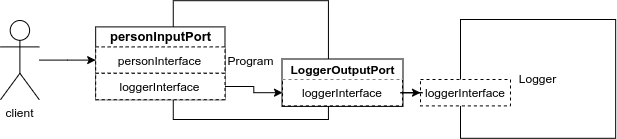
\includegraphics[width=10cm]{ExamplePort}
    \centering
    \caption{A service for port example}
    \label{list:example-port-graphic}
\end{figure}

\begin{listing}[ht]

    \lstset{language=Jolie,
        style=codeStyle,
        numbers=left,
        firstnumber=1
    }
    \begin{lstlisting}[frame=tlrb, caption= {Jolie Port declaration example}, label={list:example-port} ]{port-Jolie}
outputPort LoggerOutputPort {
    location: "socket://logger-service-location:3000"
    protocol: sodep
    interfaces: loggerInterface
}

inputPort personInputPort {
    location: "socket://localhost:3000"
    protocol: http
    interfaces: personInterface
    aggregates: Logger
}

main {
    createPerson(person)(result){
        log@LoggerOutputPort(person)
        result = true
    }
}
\end{lstlisting}
\end{listing}

In this section, we briefly show components for expressing a communication port in Jolie. Port can either be expressed as an incoming or outgoing communication. Both consist of fields that together define details for deploying a service, such as the operations and the message structure it accepts, the location it is using, and the communication protocol. Jolie is also equipped with a set of primitives that allow an advanced composition at the communication level, such as aggregation, which aggregates outgoing and incoming port, allowing the incoming port to accept and forward the message to the destination outgoing port.

\FloatBarrier


\subsubsection{Execution modality}

In the previous port decoration example at ~\ref{list:example-port}, the runtime execution terminates after service has finished the workflow of \texttt{createPerson} operation. But as a service, we would like the service to keep listening to the incoming messages without terminates after the first message has been processed.
Jolie offers a set of primitive of program execution behavior through \texttt{execution} statement which accepts three types of execution behaviors:

\begin{itemize}
    \item \textit{single}, a default behavior; which terminates the program after current process is finished.
    \item \textit{sequential}, initiate new execution behavior when the current process is finished.
    \item \textit{concurrent}, initiate new execution behavior whenever there is an operation invocation.
\end{itemize}

\begin{figure}[ht]
    \begin{framed}
        \begin{grammar}
            <executionMode>
            ::= `execution' `{' <modality> `}'

            <modality>
            ::= `single'
            \alt `concurrent'
            \alt `sequential'
        \end{grammar}
    \end{framed}
    \caption{Jolie Execution Modality Syntax}
\end{figure}

Thus, it is possible to change the service behavior in figure ~\ref{list:example-port} to accept multiple operations invocation concurrently by adding one single line of code as shown in line 5 of figure ~\ref{list:example-port-concurrent}

\begin{listing}[ht]

    \lstset{language=Jolie,
        style=codeStyle,
        numbers=left,
        firstnumber=1
    }
    \begin{lstlisting}[frame=tlrb, caption= {Jolie concurrent service example}, label={list:example-port-concurrent} ]{typeDef-Jolie}
outputPort LoggerOutputPort { ... }

inputPort personInputPort { ... }

execution {concurrent}

main {
    createPerson(person)(result){
        ...
    }
}
\end{lstlisting}
\end{listing}

\FloatBarrier

\subsubsection{Embedding Services}
\label{sec:embedded}

One of the service composition patterns widely uses is \textit{Orchestration}, which consist a central service, so-called an \say{orchestrator}, coordinates and conducts a group of services to achieve their responsibility together. The service orchestration can be achieved with ease by the embedding mechanism of Jolie; it allows multiple services to be executed in a single execution environment in a hierarchical order.
Moreover, it allows rapid communication of services via local memory communication, which delivers messages internally within the virtual machine.

The embedding mechanism expands a service into two roles, \textit{embedder} and \textit{embedded} service. The embedder conducts the services of the embedded. The mechanism allows the developer to separate a complex Jolie service into small single responsibility services that can later be reused in another project. 

The local memory communication channel can be defined by specifying a communication medium as \textit{local} in the \texttt{Location} field of the communication port.
Jolie offers a handy mechanism to embedded an external service into local execution.

Jolie supports different technologies to be embedded as a service, as it is not limited to a service defined in Jolie language. Currently, Jolie supports two additional services from external technology, which are Java and Javascript. Table ~\ref{table:embedded-technology-path} reports the list of supported technologies and the \(\langle path \rangle\) declaration a Jolie program must define to use the different supported technologies, as shown in table ~\ref{fig:embedded-syntax}

\begin{table}[h]
    \centering
    \begin{tabular}{ |c|l| }
        \hline
        Technology & Expecting content in path                                         \\
        \hline
        Jolie      & A path to a jolie file                                            \\
        Java       & A target to a java class which inherits Jolie's JavaService class \\
        Javascript & A path to a javascript file                                       \\
        \hline
    \end{tabular}
    \caption{Embedding technology and path content}
    \label{table:embedded-technology-path}
\end{table}


\begin{figure}[ht]
    \begin{framed}
        \begin{grammar}
            <embedStmt> ::= `embedded' `{' <embedTechnology> `:' ( <path> ( `in' <portName> )? )* `}'

            <embedTechnology> ::= 'Java' | 'Javascript' | 'Jolie';

            <path> ::= StringLiteral;

            <portName> ::= <ID>;

            <internalService>
            ::= 'service' <ServiceName> `{' processes `}';
        \end{grammar}
    \end{framed}
    \caption{Grammar for Jolie embedding statement}
    \label{fig:embedded-syntax}
\end{figure}

The syntax of \(\langle portName \rangle\) defined an output port name to be bound to the embedding service. There are three cases to be considered here, which is detailed in the list below:

\begin{itemize}
    \item If it is left blank, the embedding service will be launched as a standalone service.
    \item If it is pointing to an existing outputPort, the embedding service will bind a communication channel to the embedded service input ports declared \textit{`local'} in the location field.
    \item If it is pointing to a new outputPort, the embedding service will automatically create a new output port and bind communication channel to embedded service input ports declared \textit{`local'} in the location field.
\end{itemize}

The example in figure ~\ref{list:jolie-embeded} shows the usage of an embedded statement in Jolie. Here the communication protocol and the location at line 1 are not defined in code. It will be bound automatically to the communication port of embedded service before the main process starts to execute. 

\begin{listing}[ht]

\lstset{language=Jolie,
    style=codeStyle,
    numbers=left,
    firstnumber=1
}
\begin{lstlisting}[frame=tlrb]{typeDef-Jolie}
outputPort personService {
    interfaces: personInterface
}

embedded {
    Jolie: "person_service.ol" in personService
}

main {
    ... // person variable initialization omitted
    createPerson@personService(person)(result)
}
\end{lstlisting}
\caption{Jolie implementation of the embedded statement}
\label{list:jolie-embeded}
\end{listing}

\FloatBarrier



As before, we can now define a syntax for the \(<deplInstruction>\) as following.

\begin{figure}[h]
    \begin{framed}
        \begin{grammar}
            <deplInstruction> ::= <executionMode>
            \alt <outputPort>
            \alt <inputPort>
            \alt <embedStmt>
            \alt <internalService>
        \end{grammar}
    \end{framed}
    \caption{Grammar for jolie's execution modality}
    \label{fig:jolie-depl}
\end{figure}


\subsection{Behavior declaration}
\label{sec:jolie-behavior}

The behaviors in Jolie define a composition of tasks, called processes, invoked when the service receives a message matching the exposed operation or performing a sequential program. A process is essentially a program statement in other programming languages, but as it is built from a distributed system concept, Jolie processes are composed differently. Composing processes, as shown in the syntax rule \(<continuation>\) in figure ~\ref{fig:jolie-process}  uses semicolon \((;)\) to define a sequential statement and a pipe \((|)\) for a parallel statement. For example given two statement \(A\) and \(B\) if we write \(A ; B\) Jolie interprets it as \textit{`execute A then B"} while \(A | B\) as \textit{`concurrently execute A and B"}. If the continuation is not defined, the default value is a sequential composition \((;)\).

In addition to the support of basic statements as other programming languages, Jolie natively supports communication statements, consisting of two patterns, i.e., One-Way operation and Request-Response operation. As the name suggest, a One-Way operation sends a message through a port and continues, while Request-Response waits for a response message from the target port and then continues. With these concepts, a Jolie program encapsulates a whole communication procedure within a single statement. From the syntax, the \(<operationName>\), \(<outputPortName>\) are an identifier referring to the calling operation and port name respectively. In contrast, \(expr\) is a basic expression used to send and store the received data.

Another service-oriented statement supported by Jolie is a Nondeterministic Choice defined in \(<ndInputChoices>\), which determines a workflow of the service, when the accepted operation gets called. It is useful when a service is acting as a provider in the system. The workflow consists of two parts of the execution definition defined in \(<processes>\) syntax rule. Firstly, defined within square brackets scope, generally used for building a response for return to the client since it is executing upon the operation is invoked. The second one, defined after the brackets, is performed after service has responded to the client. It is useful in a situation where there are blocking tasks that exclusively contribute to the response message.

\begin{figure}[h]
    \begin{framed}
        \begin{grammar}
            <processes>
            ::= <process> ( continuation? <process> )*

            <continuation> ::= `|' \hfill (parallel composition)
            \alt `;' \hfill (sequential composition)

            <process> ::= \dots
            \alt <ndInputChoices> \hfill (non-deterministic Choice)
            \alt <inputStmt> \hfill (input operation statement)
            \alt <outputStmt> \hfill (output operation statement)

            <ndInputChoices>
            ::= <ndInputChoice>+

            <ndInputChoice>
            ::= '[' <inputStmt> `{' <processes> `}' ? ']' <processes>?

            <inputStmt>
            ::= <operationName> '(' <expr>? ')' \hfill (one-way)
            \alt
            <operationName> '(' <expr>? ')' '(' <expr>? ')' ( `{' <processes> `}' )? \hfill (request-response)

            <outputStmt>
            ::= <operationName> `@' <outputPortName> '(' <expr>? ')' \hfill (one-way)
            \alt
            <operationName> `@' <outputPortName> '(' <expr>? ')' '(' <expr>? ')' \hfill (request-response)
        \end{grammar}
    \end{framed}
    \caption{Grammar for Jolie's deployment instruction}
    \label{fig:jolie-process}
\end{figure}

Now let us look back to the Jolie service in example shown in figure ~\ref{list:example-port}, at line 15-18

\begin{lstlisting}{ndChoice}
    createPerson(person)(result){
        log@LoggerOutputPort(person)
        result = true
    }
\end{lstlisting}

The statement \texttt{createPerson(person)(result)} tells the runtime execution to wait for a receiving operation \texttt{createPerson} and assigns the receiving message to the \texttt{person} variable, then the execution proceeds with the processes defined in braced scope. After the execution in the braces finished, the value in variable \texttt{result} will be sent back to the operation caller.

\subsubsection{Procedure Definition}
\label{sec:jolie-procedure-def}

Jolie allows programmer to split process composition into a procedure, which can be invoked by calling the its name. Calling the procedure essentially tell the runtime execution to perform instruction within the caller scope. As an example at ~\ref{list:procedure}, calling \texttt{doubleX} in main scope cause \texttt{X} in the procedure to be referred to same \texttt{X} as the \texttt{main} scope. There are two types of special procedures in Jolie that define a target execution processes which are \texttt{init}, the initialization procedure, and \texttt{main}, the main execution target.

\begin{figure}[h]
	\begin{framed}
		\begin{grammar}
			<procedureDefinition> ::= `define' <ID> `{' <processes> `}'
		\end{grammar}
	\end{framed}
	\caption{Jolie Procedure Definition Syntax}
\end{figure}


\begin{listing}[h]
\lstset{language=Jolie,
	style=codeStyle
}
\begin{lstlisting}[frame=tlrb, caption= {Jolie procedure example}, label={list:procedure}]{procedure-Jolie}
define doubleX{
	X = X * 2
}

main {
	X = 5
	doubleX
	// now X == 10
}
\end{lstlisting}
\caption{Jolie procedure example}
\label{list:procedure}
\end{listing}

The \(<process>\) rule is the composition of tasks to be perform by the service, it will be discuss at \autoref{sec:jolie-behavior}.

\FloatBarrier


\subsection{Include statement}
\label{sec:jolie-include}

Jolie support modular programming via an include statement. Similarly to C programming language include directive, when the parser found an include statement, it substitutes the statement into the content of the target input file. Include statement is used for separate file into a smaller component such as the interface definition file (.iol) or used for adding a functionality of the built in library. The include statement required a string literal indicating the location of the included file. If the given path is an absolute location, Jolie will attempt to find it directly. Otherwise, the searching paths are following.

\begin{itemize}
    \item A relative path resolved from the current working directory, where the jolie interpreter is called
    \item A relative path resolved from Jolie's standard \texttt{include} library directory.
    \item A relative path resolved from paths defined by the passing command line argument.
\end{itemize}

It is worth noting that the searching path is a relative path to the current working directory, not the program itself directory.

Jolie also supports code inclusion from the achieve files.
The including target string can specify as a Java JAR url like \texttt{<scheme>:file:<location>\newline!/{entry}} where \texttt{scheme} can be either a Java archive file (\texttt{jar}) or a Jolie achieve file (\texttt{jap}), \texttt{location} is a path to the archive file, and lastly \texttt{entry} is an internal path to a target inclusion file.

\begin{figure}[h]
    \begin{framed}
        \begin{grammar}
            <includeStmt> ::= `include' StringLiteral
        \end{grammar}
    \end{framed}
    \caption{Jolie Grammar for include statement}
    \label{fig:jolie-definition}
\end{figure}

\subsection{Jolie example program}

Once we are familiar with the basic concept of Jolie, we can demonstrate an example program of Jolie service, a sum service which take two integer and sum them together. We also going demonstrate how to invoke an operation of a service.

Firstly, the interface declaration file defined a list of shared definition between the client and sum service. which are type call \texttt{intPair} and the interface defining a operation that is used for communication.

\begin{listing}[ht]
    \lstset{language=Jolie,
        style=codeStyle
    }
    \begin{lstlisting}[frame=tlrb,caption={Sum service interface}, label={list:example-iol}]{sumIface.iol}
// sumIface.iol
type intPair: void{
    x : int
    y : int
}
interface SumIface{
    requestResponse: sum(intPair)(int)
}
\end{lstlisting}
\end{listing}

Then we define the sum server shown in figure ~\ref{list:example-sum}, which capable of performing a sum operation when it is called through an input port \texttt{IP}. In line 9 of server service, we instruct the service to execute a workflow instruction when receive an invocation. Lastly in our main behavior, we create a non deterministic choice as a handler for the operation defined in \texttt{SumIface}.

\begin{listing}
    \lstset{language=Jolie,
        style=codeStyle,
        numbers=left,
        firstnumber=1
    }
    \begin{lstlisting}[frame=tlrb, caption= {Sum service}, label={list:example-sum} ]{sumservice.ol}
include "sumIface.iol" // include interface file

inputPort IP{
    location:"socket://localhost:3000"
    protocol:sodep 
    interfaces:SumIface
}

execution { concurrent }

main{
    [sum(req)(res){
        res = req.x + req.y
    }]
}
\end{lstlisting}
\end{listing}

For our example of the service's client, we firstly include the standard library `console', which exposes us the ability to perform console related tasks eg. print and receive console input. Later at line 4 we declare a communication channel called \texttt{Calculator} which bind the communication channel to server's input port. Lastly we declare a behavior of the client, we basically build a message value and send it through invoke a operation \texttt{sum} in the output port.

\begin{listing}
    \lstset{language=Jolie,
        style=codeStyle,
        numbers=left,
        firstnumber=1
    }
    \begin{lstlisting}[frame=tlrb,caption= {Sum client example}, label={list:example-client}]{client.ol}
include "console.iol" // use build-in service "console"
include "sumIface.iol" // include an interface file 

outputPort Calculator{
    location:"socket://localhost:3000"
    protocol:sodep 
    interfaces:SumIface
}

define printResult{
    println@Console(result)()
}

main{
    req.x = 2;
    req.y = 3;
    sum@Calculator(req)(result)
    printResult
}
\end{lstlisting}
\end{listing}


\subsection{Jolie implementation}

In this section we will give an introduction to the implementation of Jolie programming language. After finished this chapter, the reader should follow the implementation design and changes that had made in Jolie internal implementation for support of the module system.

The implementation of Jolie language is based on interpretation approach. Therefore, the interpreter is responsible for total life-cycle of a Jolie program; parsing a program until executing it. There are four components that working together in order to interpret a Jolie program, a parser which parse source code into an Abstract Syntax Tree (AST), each Jolie behavior statement is later transform into a tree of Jolie executable process called OOIT (Object-oriented interpretation tree), the runtime environment which store the state and the responsible for executing the process, lastly, the Communication Core (CommCore) is the foundation of communication between Jolie runtime environment.

The workflow of interpreting a Jolie source code is following:

\begin{enumerate}
    \item The command-line configuration get parsed, this include locate the executing target file.
    \item The source code get parsed in parser, where the AST is created.
    \item The program's component nodes in AST get verified it's semantic. And resolve the type link definition
    \item The interpretation tree, or the runtime executable object, is generated from AST.
    \item The CommCore is initialized from the communication ports configuration declared in AST node.
    \item The embedding services is initialized and communication related variable is set.
    \item The runtime execute init/main procedure definition process.
\end{enumerate}

Type link definition is a definition that is referred to a type that is already defined. This may in a form of \lstinline{ type A : B } where B is a type definition previously defined in the program. The abstract syntax \texttt{A} gets resolved and linked to \texttt{B} during the verification of semantic in  

\FloatBarrier


%  parse configuration


\section{Module System}

Modular programming is a programming design technique originally developed in the late 1960s by Larry Constantine, who observed that programs that were easiest to implement and changes are those composed of simple, independent modules\cite{Stevens-1999}. The problem that can be separated into pieces is faster and easier to solve, as its subproblems can be considered independently. The problem with multiple aspects to deal with simultaneously is one that found the hardest one.

As presented by the Constantine (1968)\cite{Stevens-1999}, a module is a set of one or more contiguous program statements with a name by which other parts of the system can invoke it and preferably have its own distinct set of variable names. A module can be connected to others through an interface that defines the set of names that is accessible by other modules.

A module system is a set of mechanisms that targets the decomposition of large applications into smaller pieces. It enables support of the module concept natively in a programming language. 

The import statement is the statement that is commonly used in the module system to access and retrieve a named definition in modules. It is generally responsible for locating the target module and link the target definition to the local execution environment.

Usage of terms in the module system varies between programming languages as their implementation detail of the module system. Before diving into the module's system of each selected popular programming language, the reader will be introduced with the term that is used within their context.

In the sections below, we review a module system of a prominent programming languages, the Python programming language in particular. The choice on Python made because the documentation on its history and design choices are well preserved and easy to access and it inspired our implementation of the Jolie's module system.


\subsection{Python Module System}

The Python module system history and its design choices can be traced back to Modula-3\cite{modula-3}, as its modularity concepts influenced many modern programming languages, including Python.
Python acquired the Modula-3 usage of \texttt{dot} notation for traversing modules and elements\cite{python-foreward-essay}.

The Python's module system has been gradually evolving, in the years as shown in more than the 50 proposals related to the module system in Python Enhancement Proposals (PEP) \cite{pep0}. This chapter will discuss how Python 3.0 defined its module system and its importing mechanism.

A \textbf{module} is an object with a list of python definitions and executable statements. These statements are executed during the initialization of the module. In the file system perspective, a module is a file with 'py' extension, and the module is named after the file name.

A \textbf{package} is a module which might contain sub-modules or a sub-packages.
Thus, in the file system, directories are recognized as Python packages.
In the current version of Python, the packages are categorized into two types called regular packages and namespace packages.
A \textbf{regular package} is a package that is implemented as a directory containing \textbf{\_\_init\_\_.py} file.
The directory without a \textbf{\_\_init\_\_.py} is consider as a newer type package so-called \textbf{namespace package}.
The namespace package was introduced to natively support the declaration of a module from different locations \cite{pep420}. The element in the namespace package is called a portion, which can be a set of files in a single directory or an entry in a zip file.

\subsubsection{Import Statement}

Despite there exist a few methods for a module to invoke the import mechanism, we mainly focus on Python's import statement.
A dotted separate module name can specify the location of the target module. The target symbols are used to indicate symbol name in local namespace to be referred later for import statement caller or a wildcard character.
The syntax of import statements in Python is defined as follows in figure ~\ref{fig:python-import-stmt-syntax}.

\begin{figure}[ht]
    \begin{framed}
        \begin{grammar}
            <importStmt>
            ::= <importName>
            | <importFrom>

            <importName>
            ::= `import' <dottedAsNames>

            <importFrom>
            ::= `from' ( `.' )* ( <dottedName> | `.' ) `import' ( `*' | <importAsNames> )

            <importAsNames>
            ::= <importAsName> ( `,' <importAsName> )*

            <importAsName>
            ::= <NAME> ( `as' <NAME> )?

            <dottedAsNames>
            ::= <dottedAsName> ( `,' <dottedAsName> )*

            <dottedAsName>
            ::= <dottedName> ( `as' <NAME> )?

            <dottedName>
            ::= <NAME> ( `.' <NAME> )*

            <NAME> ::= <ID>
        \end{grammar}
    \end{framed}
    \caption{Python import statement syntax }
    \label{fig:python-import-stmt-syntax}
\end{figure}

An import statement of python has two forms, it is either in form of \texttt{<importName>} and \texttt{<importFrom>} statements. Both statements create identical instructions to the module importer, choice of use is subjectively open to the developer to pick. The semantics of these two forms is different from each other in the following way.

The first form of import, \texttt{<importName>}, every \texttt{<NAME>} declared in \texttt{<dottedName>} except the last one, must be a package, while the previous \texttt{<NAME>} can only be either a module or a package; it cannot be referred to a definition symbol inside a module.

For the second form, \texttt{<importFrom>}, the item element can be a module or any definition symbol declared within the package. In this form, it performs a lookup to symbol item inside the package; if not found, it continues with an attempt to import module items. The table ~\ref{table:python-import-def} shows the translation of symbols identified in a different form of import symbol.

\begin{table}[ht]
    \centering
    \begin{tabular}{ |l|p{0.7\linewidth}| }
        \hline
        Statement                   & Element explanation                                                                                                                                                 \\
        \hline
        import item                 & \textit{item} can either be a package or a module.                                                                                                                  \\
        \hline
        import item.subitem         & \textit{item} is a package while \textit{subitem} is a module in \textit{item}.                                                                                     \\
        \hline
        from pkg import item, item2 &
        \makecell[l]
        {If \textit{pkg} is a module,                                                                                                                                                                     \\ \textit{item} and \textit{item2} are definition symbols in \textit{pkg}                                                            \\
            If \textit{pkg} is a package,                                                                                                                                                                 \\ \textit{item} and \textit{item2} can either be a module in \textit{pkg} or \\ a definition defined in \textit{pkg}.
        }                                                                                                                                                                                                 \\
        \hline
        from pkg.mod import item    & \textit{pkg} is a package and mod is a module in \textit{pkg}, while \textit{item} can be a module of \textit{mod}, or a definition symbol defined in \textit{mod}. \\
        \hline
    \end{tabular}
    \caption{Python import element definition}
    \label{table:python-import-def}
\end{table}

There are two types of import statement in Python which determine the module lookup location \cite{pep328}. Absolute import is the default behavior for an import statement, where it will perform a lookup based on the list of system module lookup path. Other types of import statements, relative import, instruct the system to perform a lookup for module relatively from the module that an import statement resides.

A useful feature that \texttt{<importFrom>} provides to Python developer is an ability to specified a module target location. If the module target is prefixed with a dot (.), it will be considered a relative import, where a dot serves as go one level up.


\subsubsection{Import Mechanism}

After the import statement's execution is completed, it results to a set of defined definitions ready to use in the caller's execution context.
To achieve this goal, Python processes import statement in two steps, during the creation of symbol table, which the importing target symbols are created the global execution scope of the import statement caller, then the runtime execution of it combines the search of the named module and the binding of the result to the importing module's symbol reference.

At the implementation level, these two operations are performed by an abstraction called \texttt{importer}, which consists of two other crucial abstraction objects: finders and loaders.
Finders are responsible for performing module lookup, while loaders use the result from the finder to execute and create a module object which later is saved to the cache.
Lastly, the loader binds names as defined in the import statement to the local execution environment.

Python locates a module with a \texttt{finder}, which is categorized into two types based on the location where the finder should attempt to find the module.
Firstly the \texttt{MetaPathFinder} will perform a lookup on a list of paths passing through the finding method.
The second type of finder, the \texttt{PathEntryFinder}, performs a look-up only on at a list of paths to the path that is assigned during its creation.
Searching operations may cause certain side-effects to the execution environment. In case of importing a module inside the package, it is processed by importing each parent packages from top-level until the module is reached, which means it also executes the initialization instructions of every module target's parent packages.

After the module has been loaded into the execution environment, the importing target symbols are binding to the importer global execution scope; this scope is also called the module scope. There is only a single global scope in the Python program execution.

\subsubsection{Symbol Privacy}

In Python, every declaration of the symbol is considered a private symbol if it having a prefixed underscore (\_). Such a symbol will be ignored for a wildcard import (from ... import *), and an error will be raised when it is implicitly referred to, as the declaration can only be used in its module scope.

